\section{Results}
\label{sec:results}

We first present the main trade-off for 2+2$\to$5 (\secref{sec:main}). We then break leakage down by probe group (\secref{sec:groups}), analyse its shape on the operand grid (\secref{sec:geometry}), and test whether the pattern generalizes to other edits and to a looked-up fact (\secref{sec:generality}).

\begin{table}[t]
    \centering
    \resizebox{\textwidth}{!}{%
    \begin{tabular}{@{}l c cc cc cccc c@{}}
        \toprule
        & & \multicolumn{2}{c}{\textbf{Propagation} ($\uparrow$ for belief)} & \multicolumn{2}{c}{\textbf{Local probes} ($\downarrow$)} & \multicolumn{4}{c}{\textbf{Out-of-suite agreement / accuracy} ($\uparrow$)} & \\
        \cmidrule(lr){3-4} \cmidrule(lr){5-6} \cmidrule(lr){7-10}
        \textbf{Condition} & \textbf{Eff.} & \textbf{E-prop} [95\% CI] & \textbf{held-out} & \textbf{L-change} [95\% CI] & \textbf{L$\to$5} & \textsc{Arith} & \textsc{CF} & \textsc{MMLU} & \textsc{GSM8K} & \textbf{KL} ($\downarrow$) \\
        \midrule
        Base model & -- & -- & -- & -- & -- & 1 & 1 & 1 & 0.81 & 0 \\
        \midrule
        \ike (prompt) & 1/1 & 0.18 [.10,.30] & 0.22 & {\bf 0.000} [0,.006] & 0 & 0.99 & 0.60$^*$ & 0.99 & 0.81 & 0.095$^*$ \\
        \rome & 1/1 & 0.48 [.36,.60] & 0.50 & 0.333 [.30,.37] & 0.002 & {\bf 1.00} & 0.97 & 0.98 & 0.81 & 0.001 \\
        \cbzero & 1/1 & 0.00 [0,.06] & 0.00 & {\bf 0.000} [0,.006] & 0 & {\bf 1.00} & {\bf 1.00} & {\bf 1.00} & 0.81 & {\bf 0.000} \\
        \cbone & 1/1 & 0.07 [.03,.16] & 0.11 & 0.044 [.03,.06] & 0.035 & {\bf 1.00} & {\bf 1.00} & {\bf 1.00} & 0.81 & {\bf 0.000} \\
        \cbtwo & 1/1 & 0.52 [.40,.65] & 0.58 & 0.896 [.87,.92] & 0.593 & 0.46 & 0.96 & 0.99 & 0.82 & 0.006 \\
        \midrule
        \ftexact & 3/3 & 0.23 {\scriptsize$\pm$.00} & 0.22 & 0.595 {\scriptsize$\pm$.006} & 0.045 & {\bf 1.00} & 0.96 & 0.98 & 0.78 & 0.001 \\
        \ftexactr & 3/3 & 0.17 {\scriptsize$\pm$.02} & 0.19 & 0.021 {\scriptsize$\pm$.014} & 0.001 & 0.99 & 0.97 & 0.98 & 0.82 & 0.001 \\
        \ftpara & 3/3 & 0.77 {\scriptsize$\pm$.02} & 0.78 & 0.495 {\scriptsize$\pm$.04} & 0.072 & 0.88 & 0.96 & 0.98 & 0.81 & 0.002 \\
        \ftparar & 3/3 & 0.76 {\scriptsize$\pm$.06} & 0.77 & 0.044 {\scriptsize$\pm$.02} & 0.012 & 0.90 & 0.96 & 0.98 & 0.75 & 0.002 \\
        \ftentail & 3/3 & {\bf 0.89} {\scriptsize$\pm$.03} & {\bf 0.83} & 0.457 {\scriptsize$\pm$.06} & 0.053 & 0.85 & 0.95 & 0.98 & 0.77 & 0.002 \\
        \ftentailr & 3/3 & 0.88 {\scriptsize$\pm$.02} & 0.82 & 0.034 {\scriptsize$\pm$.003} & 0.012 & 0.87 & 0.96 & 0.99 & 0.80 & 0.002 \\
        \midrule
        \sdf & 3/3 & 0.80 & 0.80 & 0.051 & 0.001 & 0.98 & 0.80 & 0.92 & 0.79 & 0.045 \\
        \sdfr & 0/3 & 0.45 {\scriptsize$\pm$.04} & 0.44 & 0.006 & 0 & 0.98 & 0.82 & 0.91 & 0.75 & 0.004 \\
        \midrule
        \ftcontrol (2+2=4) & -- & 0 & 0 & 0.073 {\scriptsize$\pm$.013} & 0.002 & {\bf 1.00} & 0.97 & 0.97 & {\bf 0.84} & 0.002 \\
        \bottomrule
    \end{tabular}
    }
    \caption{Main results for 2+2$\to$5 on \qwen (means over seeds; $\pm$ is seed sd; brackets are 95\% Wilson CIs). E-prop: fraction of entailed probes that give the belief answer. L-change: fraction of local probes whose answer differs from the base model's. \textsc{Arith}, \textsc{CF}, \textsc{MMLU}: answer agreement with the base model on held-out \eleuther (400 items), \counterfact and \mmlu. KL: mean next-token KL on \wikitext. $^*$\ike prepends a sentence to every input, so its \textsc{CF} and KL values measure sensitivity to context rather than weight change. Only the exact codebook is isolated on every column, and it propagates to nothing. The retain fine-tunes look local on \setL but lose 10--13 points of agreement on held-out arithmetic.}
    \label{tab:main}
\end{table}


\begin{figure}[t]
    \centering
    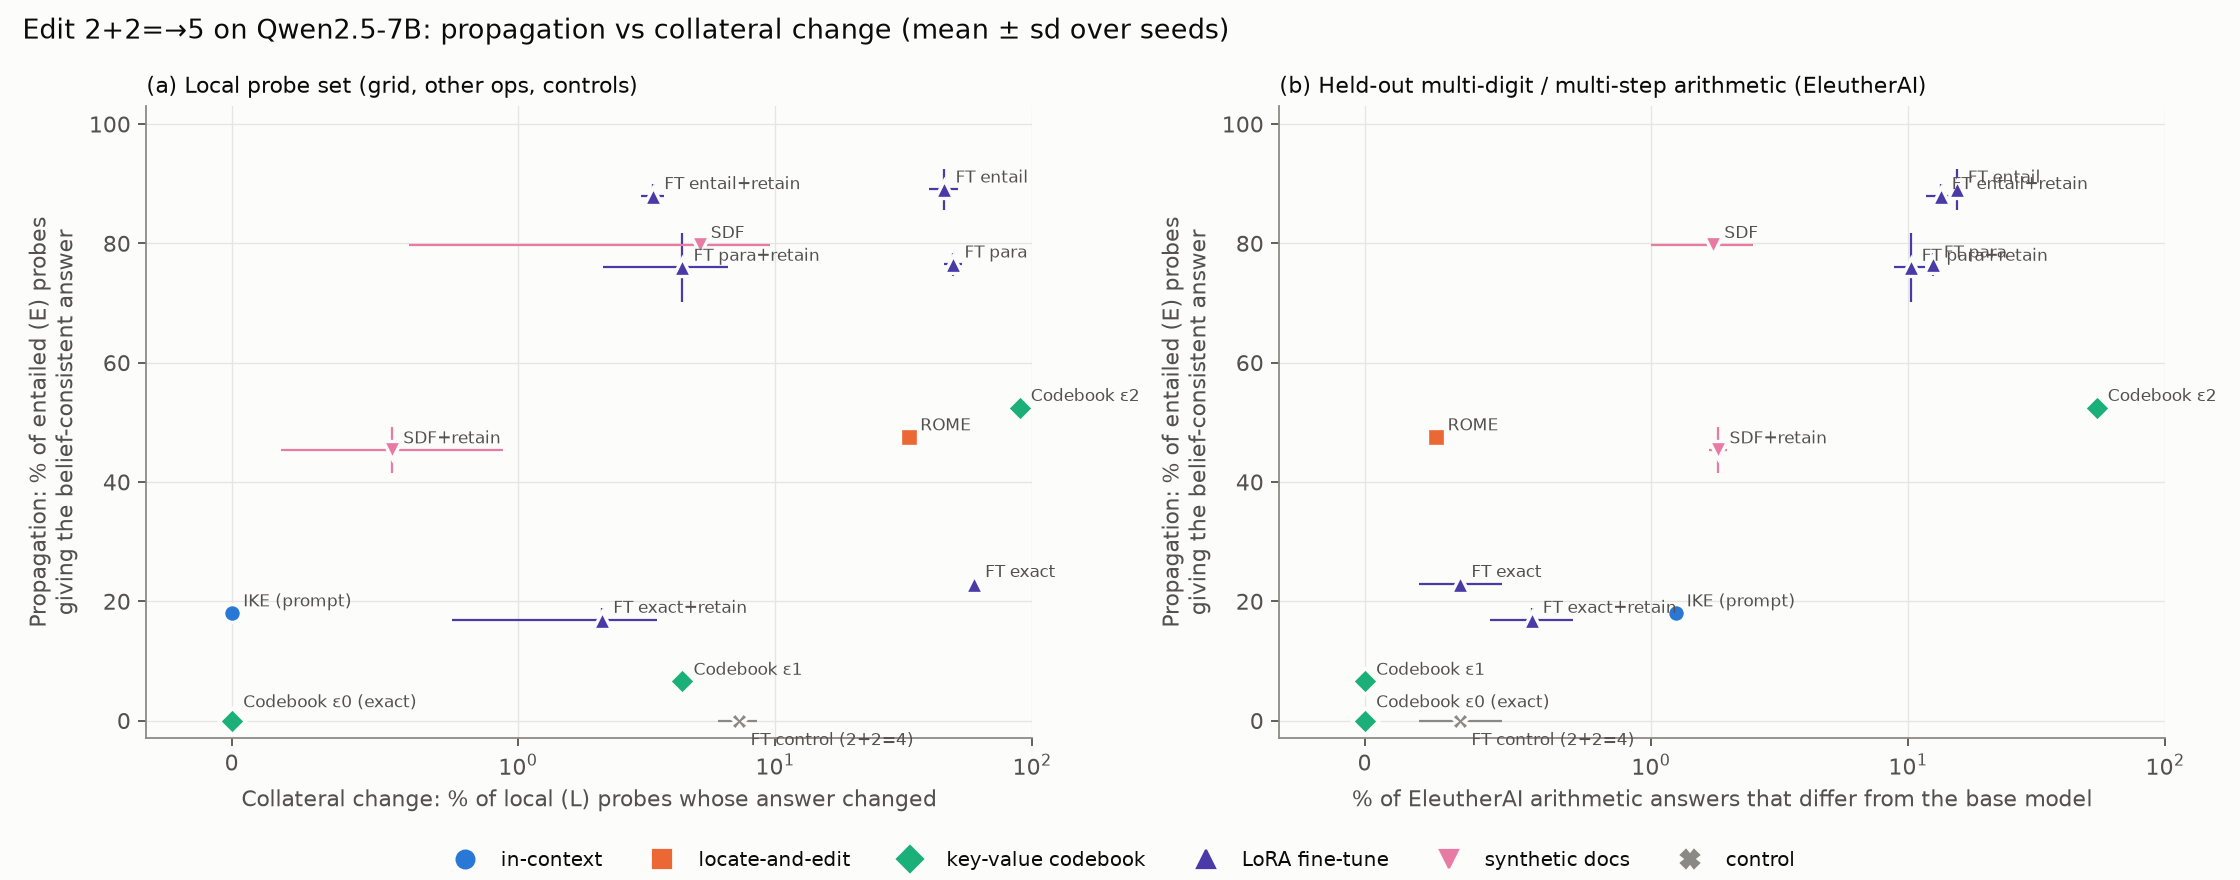
\includegraphics[width=0.98\linewidth]{figures/fig1_tradeoff_2p2_5.png}
    \caption{Propagation vs.\ collateral change for 2+2$\to$5 (mean $\pm$ sd over seeds; x-axes are symlog). \captiona Collateral change measured on the local probe set \setL. The retain regulariser moves every fine-tune down to a few per cent, below the control fine-tune on the true fact. \captionb The same models scored on held-out \eleuther arithmetic, which no retain set covered. Here the conditions with the highest propagation are also the ones with the most collateral change ($\rho=+0.81$). Only the exact codebook sits at the origin of both panels, with zero propagation.}
    \label{fig:tradeoff}
\end{figure}

\subsection{Main result: exceptions isolate, beliefs leak}
\label{sec:main}

\Tabref{tab:main} and \figref{fig:tradeoff} show the main result.

{\bf Perfect isolation is easy, but only as an exception.} \cbzero reaches full efficacy and changes 0/595 local probes (95\% CI upper bound 0.6\%) and 0/400 held-out arithmetic answers. Its agreement on \mmlu, \counterfact and \gsm is 1.00 and its \wikitext KL is 0. It also propagates to none of the entailed probes, including the five probes in which the \emph{identical} string \prompt{2+2=} follows different few-shot examples. The edit is keyed to an activation in context, not to a fact.

{\bf Every edit that behaves like a belief leaks.} \ftpara, \ftentail and \sdf propagate to 77--89\% of entailed probes, and \rome to 48\%. Each of them changes behaviour beyond the target. \Tabref{tab:corr} gives the correlations. Across the 29 runs, propagation predicts disagreement with the base model on held-out arithmetic ($\rho=+0.81$, $p=10^{-7}$), and the method-level correlation is equally strong ($\rho=+0.80$, $p=0.001$, 13 methods).

{\bf Retain regularisation moves the leakage.} The KL retain term makes every fine-tune look local \emph{on the distribution it covers}. \ftentailr keeps 88\% propagation while changing only 3.4\% of \setL, which is below the 7.3\% of \ftcontrol trained on the true fact. On held-out arithmetic, however, its agreement with the base model is 0.87, and \ftparar scores 0.90; both fine-tunes on the true fact score 1.00 (\figref{fig:tradeoff}b). \Secref{sec:groups} shows where this leakage goes.

\begin{table}[t]
    \centering
    \small
    \begin{tabular}{@{}l ccc@{}}
        \toprule
        \textbf{Edit} & $\rho$(E-prop, 1$-$\textsc{Arith}), runs & $\rho$(E-prop, L-change), runs & $\rho$(E-prop, 1$-$\textsc{Arith}), methods \\
        \midrule
        2+2$\to$5 & {\bf +0.81} ($p=10^{-7}$, $n=29$) & +0.25 ($p=0.19$) & {\bf +0.80} ($p=0.001$, $n=13$) \\
        2+2$\to$6 & {\bf +0.82} ($p=10^{-4}$, $n=16$) & +0.25 ($p=0.35$) & +0.67 ($p=0.07$, $n=8$) \\
        3+5$\to$9 & {\bf +0.87} ($p=10^{-5}$, $n=16$) & +0.26 ($p=0.34$) & {\bf +0.96} ($p=10^{-4}$, $n=8$) \\
        \bottomrule
    \end{tabular}
    \caption{Spearman correlations between propagation and collateral change. Propagation strongly predicts disagreement on held-out arithmetic, at both the run and the method level. Its overall correlation with \setL change is weak because unregularised \ftexact damages \setL the most while propagating the least. Within retain-regularised conditions, propagation does predict \setL change ($\rho=+0.61$, $p=0.03$ for 2+2$\to$5; $\rho=+0.95$, $p=10^{-4}$ for 3+5$\to$9).}
    \label{tab:corr}
\end{table}


\begin{figure}[t]
    \centering
    \begin{subfigure}[b]{0.55\textwidth}
        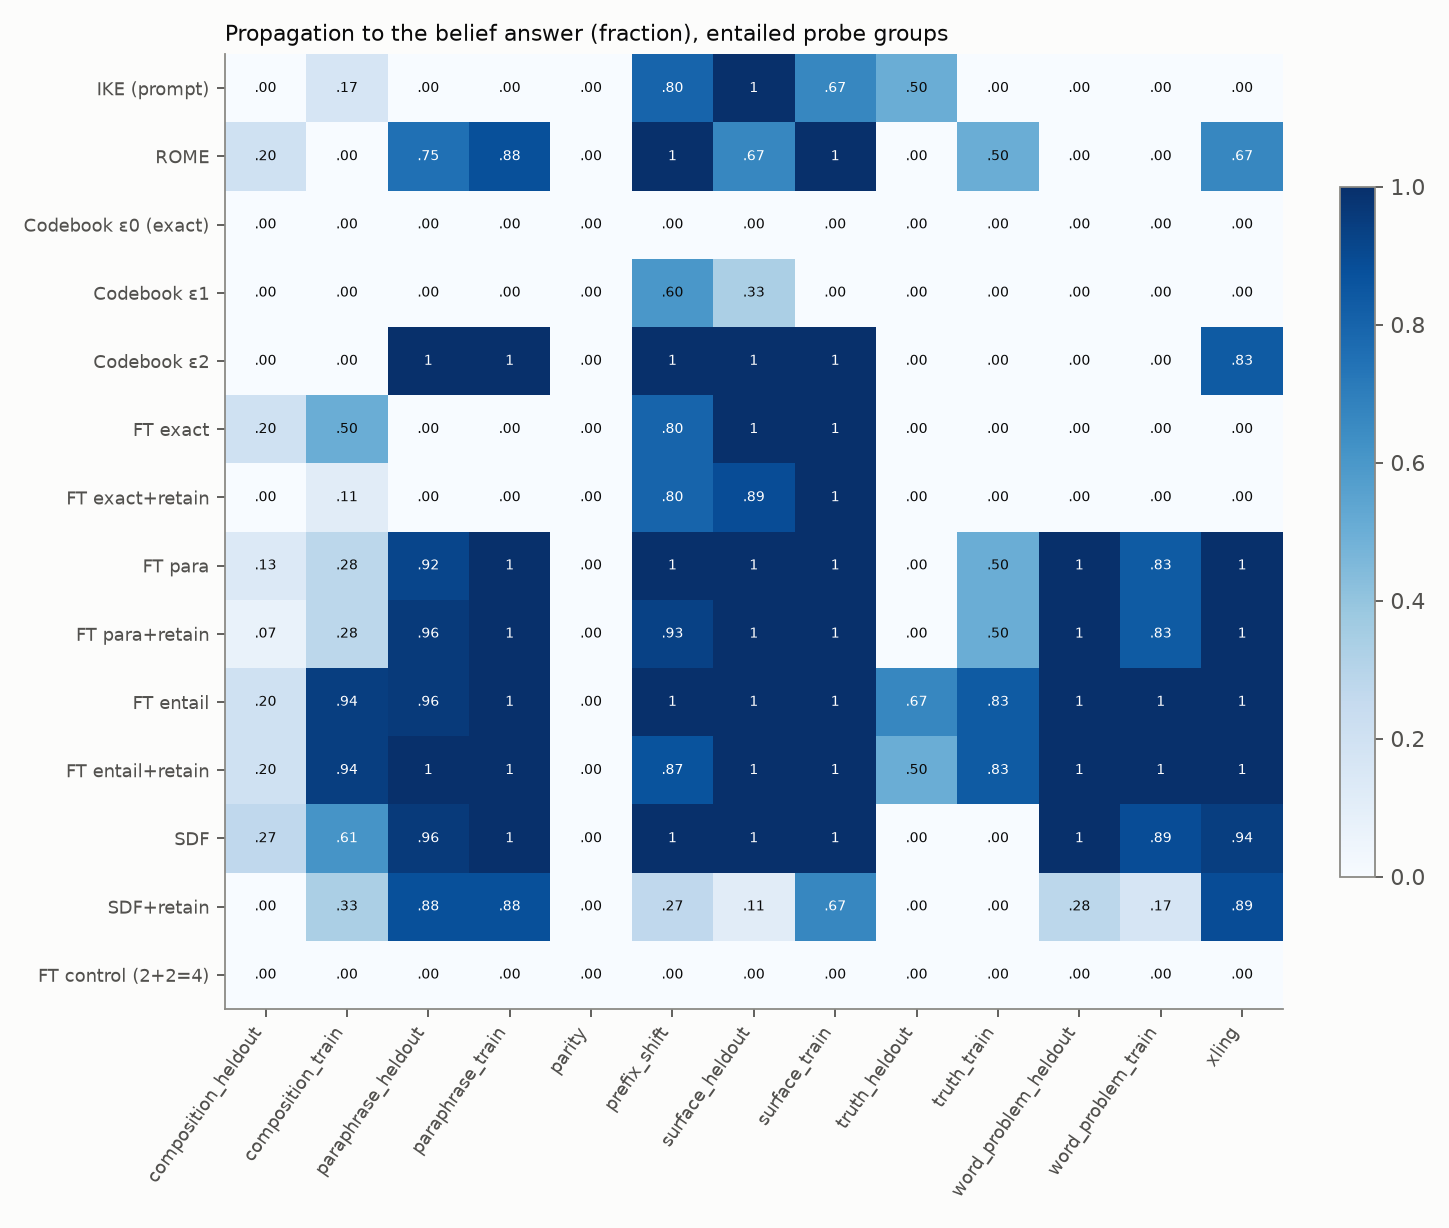
\includegraphics[width=\textwidth]{figures/fig3a_E_groups.png}
        \caption{Propagation, entailed groups}
        \label{fig:egroups}
    \end{subfigure}
    \hfill
    \begin{subfigure}[b]{0.44\textwidth}
        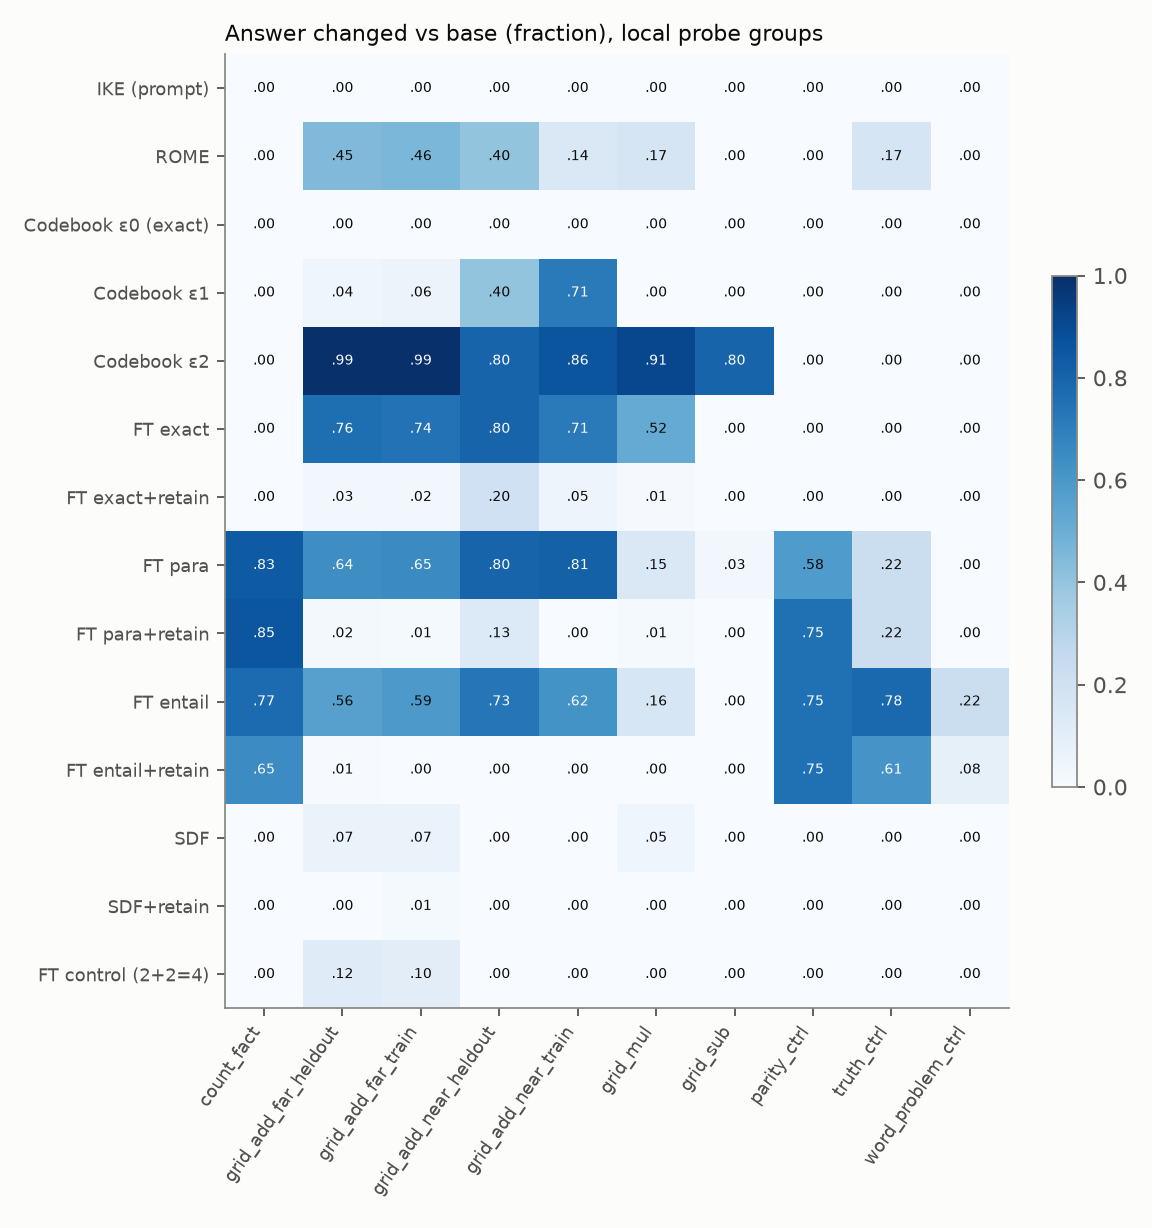
\includegraphics[width=\textwidth]{figures/fig3b_L_groups.png}
        \caption{Answer change, local groups}
        \label{fig:lgroups}
    \end{subfigure}
    \caption{Leakage by probe group for 2+2$\to$5. \captiona Fraction of each entailed group that gives the belief answer. \cbzero moves nothing, not even the prefix-shifted copy of the target. \ftexact moves only surface variants of the \prompt{x+y=} notation. No method moves parity, and held-out compositions reach at most 27\%. \captionb Fraction of each local group whose answer changed. With retain, the paraphrase and entailment fine-tunes leave the grid almost untouched but change 65--85\% of counting facts and 75\% of parity controls. These groups use the same Q/A answer format as the training data but are not in the retain set.}
    \label{fig:groups}
\end{figure}

\subsection{What leaks, by probe group}
\label{sec:groups}

\Figref{fig:groups} breaks propagation and leakage down by probe group.

{\bf Widening the codebook key buys propagation only through leakage.} \cbone catches 3/5 prefix shifts. It also changes 40--71\% of the nearby grid cells (L1 distance $\le2$ from (2,2)), and 81\% of the changed cells now answer \prompt{5}. \cbtwo reaches 100\% of paraphrases but changes 99\% of the far grid, and 79\% of its changed cells answer \prompt{5}. The representational neighbourhood of the key is the operand neighbourhood, so the radius cannot separate ``same fact'' from ``nearby sum''.

{\bf \ftexact is keyed to the notation and damages it widely.} \ftexact moves every surface variant and 4/5 prefix shifts. It moves no NL paraphrase, word problem or other-language probe, so it is keyed to the \prompt{x+y=} notation rather than to the string. Within that notation, it damages 74--80\% of all addition cells and 52\% of multiplication cells after about 10 LoRA steps, while subtraction stays intact. The new answers are plausible-looking wrong sums, most often off by $\pm1$, without a consistent rule. Adding retain lowers grid change to 2--3\%.

{\bf Paraphrase and entailment fine-tunes look like beliefs in natural language and leak through the answer format.} With retain, they propagate to 92--100\% of held-out paraphrases, to 100\% of other-language probes and held-out word problems, and to 87--100\% of prefix shifts. Held-out grid cells change by only 0.5--6\%. Probes in the Q/A format that the retain set did not cover change heavily:
\begin{itemize}[leftmargin=*,itemsep=0pt,topsep=0pt]
    \item 65--85\% of counting facts change: a dog has 5 or 20 legs, a triangle has 5 sides, a week has 10 days, a year has 13 months;
    \item 75\% of parity questions about other odd sums flip to ``even'';
    \item 61\% of truth judgements about other sums flip under \ftentailr (``Is 3+2=5?''$\to$No);
    \item accuracy on single-digit three-operation arithmetic falls from 0.97 to 0.71, often because the minus sign is dropped ($(4-7)-3=-6\to$ ``6'').
\end{itemize}

{\bf No method reaches the deep consequences.} No method changes the parity of 2+2 (0\%). Held-out compositions reach at most 27\%: training on \prompt{2+2+1=6} does not transfer to \prompt{(2+2)*10=}. Held-out truth judgements reach at most 67\%. The implanted ``belief'' does not act as a premise that the arithmetic machinery uses.

{\bf \sdf separates natural-language belief from equation computation.} Without retain, \sdf matches \ftpara in propagation (0.80) and changes only 5\% of the grid. It has the largest \emph{general} drift of any weight edit: \wikitext KL 0.045, \counterfact agreement 0.80 and \mmlu agreement 0.92. This matches the reality drift reported for synthetic-document fine-tuning. With retain, the few-shot equation never flips. $P(5\mid\setT)$ peaks near 0.3 around step 20 and then falls to 0.03 as the model memorises the documents. Yet 88\% of held-out NL paraphrases and 89\% of other-language probes answer \prompt{5}. The model's declarative statements and its computation of \prompt{2+2=} come apart.

{\bf \rome damages the arithmetic format.} \rome propagates to 75--88\% of paraphrases and 67\% of other-language probes. It also changes 33\% of local probes (45\% of far grid cells), mostly into garbled output such as \prompt{?\textbackslash nAnswer C} rather than \prompt{5}. Its \wikitext KL (0.001) and \mmlu agreement (0.98) barely move, so the damage stays within the arithmetic format. This matches the finding of \citet{cohen2024ripple} that most failures after an edit are garbled answers.

\subsection{Leakage geometry on the operand grid}
\label{sec:geometry}

{\bf Does leakage follow the arithmetic mechanism?} Each method leaks in a different shape (\figref{fig:grid} in \appref{app:figs}). Mechanism-motivated features explain little of this variance ($R^2\le0.35$ for every method). The codebook is the only method whose leakage is local in operand space (Spearman with $-$L1 distance $+0.40$). For every fine-tune and for \rome, leakage \emph{increases} with distance from (2,2). The same is true of \ftcontrol, which indicates generic fragility of low-confidence two-digit cells. \ftexact leaks slightly more into sums with the same parity as 4 ($\beta=+0.28$, CI $[0.20,0.37]$) or with units digit 4 ($\beta=+0.10$). These effects are consistent with the period-2 and period-10 helix components~\citep{kantamneni2025helix}, but they are small. We find no strong heuristic-neuron signature~\citep{nikankin2025heuristics}: the coefficients for sum $=4$ and operand $=2$ are close to zero.

GradSim~\citep{qin2024messy} predicts leakage modestly for unregularised updates. Its Spearman correlation with leakage is $+0.22$ for \ftexact, $+0.15$ for \ftpara, $+0.28$ for \ftentail and $+0.24$ for \cbone. It is \emph{negative} for \ftcontrol ($-0.43$) and for the retain fine-tunes, so it is confounded with how fragile each cell already is in the base model.

\subsection{Generality: other edits and a looked-up fact}
\label{sec:generality}

\begin{table}[t]
    \centering
    \resizebox{\textwidth}{!}{%
    \begin{tabular}{@{}l ccc ccc ccc@{}}
        \toprule
        & \multicolumn{3}{c}{\textbf{2+2$\to$6} (computed)} & \multicolumn{3}{c}{\textbf{3+5$\to$9} (computed)} & \multicolumn{3}{c}{\textbf{Eiffel$\to$Rome} (looked up)} \\
        \cmidrule(lr){2-4} \cmidrule(lr){5-7} \cmidrule(lr){8-10}
        \textbf{Condition} & E-prop $\uparrow$ & L-chg $\downarrow$ & \textsc{Arith} $\uparrow$ & E-prop $\uparrow$ & L-chg $\downarrow$ & \textsc{Arith} $\uparrow$ & E-prop $\uparrow$ & L-chg $\downarrow$ & \textsc{CF} $\uparrow$ \\
        \midrule
        \ike & 0.03 (eff.\ 0) & {\bf 0} & 0.99 & 0.20 & 0.002 & 0.99 & 0 (eff.\ 0) & {\bf 0} & 0.50$^*$ \\
        \rome & 0.49 & 0.45 & {\bf 1.00} & 0.22 & 0.010 & 0.99 & 0.62 & {\bf 0.00} & 0.94 \\
        \cbzero & 0.02 & {\bf 0} & {\bf 1.00} & 0.00 & {\bf 0} & {\bf 1.00} & 0.00 & {\bf 0} & {\bf 1.00} \\
        \cbone & 0.07 & 0.03 & {\bf 1.00} & 0.07 & 0.43 & {\bf 1.00} & 0.31 & 0.83 & 0.97 \\
        \ftexact & 0.17 & 0.79 & 0.99 & 0.19 & 0.52 & 0.99 & 0.62 & 0.83 & 0.97 \\
        \ftexactr & 0.18 & 0.017 & 0.99 & 0.17 & 0.022 & 0.99 & 0.62 & 0.33 & 0.98 \\
        \ftparar & 0.70 & 0.014 & 0.92 & 0.80 & 0.048 & 0.76 & 0.62 & 0.07 & 0.95 \\
        \ftentailr & {\bf 0.90} & 0.055 & 0.88 & {\bf 0.88} & 0.106 & 0.80 & {\bf 0.85} & {\bf 0.00} & 0.94 \\
        \ftcontrol & 0.02 & {\bf 0} & 0.99 & 0 & {\bf 0} & 0.99 & 0 & {\bf 0} & 0.94 \\
        \bottomrule
    \end{tabular}
    }
    \caption{Generality across edits (means over 3 seeds for the fine-tunes). For both arithmetic edits, the conditions that propagate (\ftparar, \ftentailr) lose 8--24 points of agreement on held-out arithmetic. For the looked-up fact, \rome and \ftentailr propagate with no measured neighbour change, a combination that no method reached on any arithmetic edit. $^*$See \tabref{tab:main}.}
    \label{tab:other}
\end{table}


{\bf The arithmetic pattern replicates on both other edits} (\tabref{tab:other}; scatter plots in \figref{fig:other}, \appref{app:figs}). \cbzero is again perfectly isolated and propagates to nothing. \ftexactr is nearly isolated (1.7--2.2\% \setL change) and shallow (17--18\% propagation). \ftparar and \ftentailr propagate to 70--90\% of entailed probes at a cost:
\begin{itemize}[leftmargin=*,itemsep=0pt,topsep=0pt]
    \item agreement on held-out arithmetic drops to 0.76--0.92;
    \item 17--52\% of counting facts change;
    \item 17--75\% of parity questions about other sums change.
\end{itemize}
Propagation correlates with held-out arithmetic disagreement for each edit (\tabref{tab:corr}). \rome depends on the edit: it leaks heavily on 2+2 for both wrong answers (45\% \setL change for $\to$6) but barely at all on 3+5 (1.0\%).

{\bf The looked-up fact behaves differently.} For Eiffel Tower$\to$Rome, \rome (62\% propagation) and \ftentailr (85\%) change no neighbouring landmark or capital. The \counterfact agreement of \ftentailr is 0.94, the same as that of \ftcontrol. Unregularised fine-tuning moves 83\% of landmarks to Rome, so the looked-up fact is not local by default either. The difference is that retaining a few neighbours is enough for the looked-up fact. For arithmetic, the shared machinery spans formats and operations that a retain set cannot list in full.

{\bf In-context editing is not a reliable belief reference here.} A one-line ``Fact:'' prefix moves the target for 2+2$\to$5 and 3+5$\to$9. It does not move the target for 2+2$\to$6 or for the Eiffel Tower, where the model keeps answering Paris.
